\documentclass[12pt]{article}
\usepackage{amssymb,amsmath,natbib,graphicx,amsthm,
  setspace,sectsty,anysize,times,dsfont,enumerate}

\usepackage[svgnames]{xcolor}

\usepackage{lscape,arydshln,relsize,rotating,multirow}
\usepackage{caption}
\captionsetup{%
  font=small,
  labelfont=normalfont,
  singlelinecheck=false,
  justification=justified
}
\usepackage{algorithm,algorithmic}

\graphicspath{{graphs/}}
\newtheorem{prop}{\sc Proposition}[section]
\newtheorem{theorem}{\sc Theorem}[section]
\newtheorem{definition}{\sc Definition}[section]
\newtheorem{lemma}{\sc Lemma}[section]
\newtheorem{corollary}{\sc Corollary}[section]

\marginsize{1.1in}{.9in}{.3in}{1.4in}

\newcommand{\nb}{\color{blue}}
\newcommand{\dbl}{\setstretch{1.5}}
\newcommand{\sgl}{\setstretch{1.2}}

\newcommand{\bs}[1]{\boldsymbol{#1}}
\newcommand{\mc}[1]{\mathcal{#1}}
\newcommand{\mr}[1]{\mathrm{#1}}
\newcommand{\bm}[1]{\mathbf{#1}}
\newcommand{\ds}[1]{\mathds{#1}}
\newcommand{\indep}{\perp\!\!\!\perp}
\DeclareMathOperator*{\argmin}{argmin}
\newcommand{\norm}[1]{|\!|#1|\!|_{1}}
\newcommand{\code}[1]{{\smaller\sf#1}}
\newcommand{\e}[1]{{\footnotesize$\times10$}{$^{#1}$}}

\usepackage[bottom,hang,flushmargin]{footmisc}

\pdfminorversion=4
\begin{document}

\sgl 

\pagestyle{empty}

~
\vskip 3cm

\noindent {\LARGE \bf One-step estimator paths for concave regularization} 

\vskip 1cm

\noindent{\Large Matt Taddy}

{\large
\vskip .5cm \noindent
{The  University of Chicago Booth School of Business}\\
\texttt{faculty.chicagobooth.edu/matt.taddy}}



\vskip 2cm

{\noindent 
The statistics literature of the past 15 years has established many favorable
 properties for sparse diminishing-bias regularization: techniques which can
 roughly be understood as providing estimation under penalty functions
 spanning the range of concavity between $L_0$ and $L_1$ norms.  However,
 lasso $L_1$-regularized estimation remains the standard tool for industrial
 `Big Data' applications because of its minimal computational cost and the
 presence of easy-to-apply rules for penalty selection.   In response, this
 article proposes a simple new algorithm framework that requires no more
 computation than a lasso path: the path of one-step estimators (POSE) does
 $L_1$ penalized regression estimation on a grid of decreasing penalties, but
 adapts coefficient-specific weights to decrease as a function of the
 coefficient estimated in the previous path step.  This provides sparse
 diminishing-bias regularization at no extra cost over the fastest lasso
 algorithms. Moreover, our `gamma lasso' implementation of POSE is accompanied
 by a reliable heuristic for the fit degrees of freedom, so that
 standard information criteria can be applied in penalty selection. The
 methods are illustrated in extensive simulations and in application of
 logistic regression to evaluating the performance of hockey players.
}


\newpage
\dbl
\pagestyle{plain}
\vskip 1cm
\section{Introduction}
\label{intro}

For regression in high-dimensions, it is useful to regularize estimation
through a penalty on coefficient size.   $L_1$  regularization \citep[i.e.,
the lasso of][]{tibshirani_regression_1996} is especially popular, with costs
that are non-differentiable at their minima and can lead to  coefficient
solutions of exactly zero.  A related approach is concave penalized
regularization (e.g. SCAD from \citealt{fan_variable_2001} or MCP from
\citealt{zhang_nearly_2010}) with cost functions that are also spiked at zero
but flatten for large values (as opposed to the constant increase of an $L_1$
norm).  This yields sparse solutions where  large non-zero values are estimated
with little bias. 

The combination of  \textit{sparsity} and \textit{diminishing-bias} 
 is appealing in many settings, and a large literature on concave
penalized estimation has developed over the past 15 years.  For example, many
authors (e.g., from \citealt{fan_variable_2001} and
\citealt{fan_nonconcave_2004})  have contributed work on their \textit{oracle
properties}, a class of results showing conditions under which coefficient
estimates through concave penalization, or in related schemes, will be the
same as if you knew the sparse `truth' (either asymptotically or with high
probability).   From an information compression perspective,  the increased
sparsity encouraged by diminishing-bias penalties (since single large
coefficients are allowed to account for the signals of other correlated
covariates) leads to lower memory, storage, and communication requirements.
Such savings are very important in distributed  computing schemes
\citep[e.g.,][]{taddy_distributed_2015}.


Unfortunately,  exact solvers for concave penalized estimation  all require
significantly more compute time than a standard lasso.  This has precluded their use in settings -- e.g., text or web-data analysis
-- where both $n$ (the number of observations) and $p$ (covariate dimension)
   are very large. As we review in Section \ref{sec:weighted},  recent
   literature recommends the use of approximate solvers. These approximations
   take the form of iteratively-weighted-$L_1$ regularization, where the
   coefficient-specific weights are based upon results from previous iterations
   of the approximate solver.  Work on one-step estimation (OSE), e.g. by
   \cite{zou_one-step_2008}, shows that even a single step of such
   weighted-$L_1$ regularization is enough to get solutions that are close to
   optimal, so long as the pre-estimates are
\textit{good enough} starting points. The crux of success is  finding starts that are, indeed, good enough.




\begin{figure*}[tbh]
\vskip -.25cm
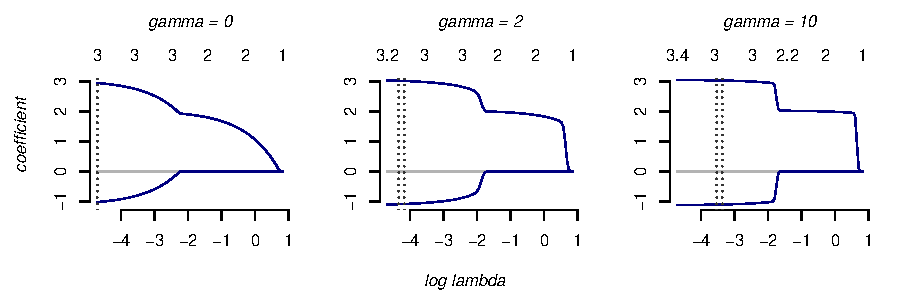
\includegraphics[width=\textwidth]{graphs/gamlr_eg}
\vskip -.25cm
\caption{\label{gamlr_eg} Gamma lasso estimation on $n=10^3$ 
 observations of $y_i = 4 + 3x_{1i} - x_{2i} + \varepsilon_i$, where
$\varepsilon_i \stackrel{ind}{\sim} \mr{N}(0,1)$ and
$\{x_{1i},x_{2i},x_{3i}\}$ are marginally standard normal with correlation of
0.9 between covariates ($x_{3i}$ is spurious). The penalty path has $T=100$
segments, $\lambda^1 = n^{-1}\left| \sum_i x_{1i}y_i\right|$, and
$\lambda^{100} = 0.01\lambda^1$. Degrees of freedom are on top and vertical
lines mark AICc and BIC selected models (see Section
\ref{sec:select}).}
\vskip -.25cm
\end{figure*}


This article provides a complete framework for sparse diminishing-bias
regularization that combines ideas from OSE with the concept of a
\textit{regularization path} -- a general technique, most famously associated
with the LARS algorithm \citep{efron_least_2004}, that estimates a sequence of
models under decreasing amounts of regularization.  So long as the estimates do not change too quickly along the path, such  algorithms can be very fast to run and are an efficient way to obtain a high-quality \textit{set} of models to choose amongst.  

A path of one-step estimators (POSE; Algorithm \ref{posealgo})
provides $L_1$ penalized regression  on a grid of decreasing
penalties, but adapts coefficient-specific weights to decrease as a function
of the coefficient estimated in the previous path step.  POSE takes advantage
of the natural match between path algorithms and one-step estimation: OSE
relies upon inputs being close to the optimal solution, which is precisely the
setting where path algorithms are most efficient.  We formalize `close' with a novel result in Theorem \ref{thm:sparseapprox} that relates weighted-$L_1$ to $L_0$ regularization.

This framework allows us to provide 
\begin{itemize}
\item a {\it path} of coefficient fits, each element of which corresponds to sparse diminishing-bias regularization estimation under a different level of penalization; where
\item obtaining the path of coefficient fits requires no more computation than  a state-of-the-art $L_1$ regularization path algorithm; and
\item there are reliable closed-form rules for selection of the optimal penalty level along this path.
\end{itemize}
The last capability here is derived from a Bayesian interpretation for our \textit{gamma lasso} implementation of POSE from which we are able to construct heuristic information criteria for penalty selection.
We view such tools as an essential ingredient for practical applicability in large-scale industrial machine learning where, e.g., cross-validation is not always viable or advisable.


The remainder of this paper is outlined as follows.  Section \ref{sec:algos}
presents the general regularized regression problem and introduces POSE, our
path of one-step estimators algorithm, and the gamma lasso (GL), our
implemented version of POSE.  Section \ref{sec:weighted} gives an overview on
the relationship between concave and weighted-$L_1$ regularization. Section \ref{sec:select} provides a Bayesian model interpretation
for the gamma lasso, and derives from this model a set of information criteria
that can be applied in penalty selection along the regularization path.
Finally, we present two empirical studies:
an extensive  simulation experiment in Section \ref{sec:sim}, and in Section \ref{sec:nhl} we investigate the data analysis question: given all goals in the past decade of NHL hockey, what can we say about individual player contributions? 


\section{Paths of one-step estimators}
\label{sec:algos}

Denote $n$ response observations as $\bm{y} = [y_1,\ldots,y_n]'$ and the associated matrix of $p$ covariates as $\bm{X} =
[\bm{x}_1 \cdots \bm{x}_n]'$, with rows $\bm{x}_i = [x_{i1},\ldots,x_{ip}]'$ and columns $\bs{x}_j = [x_{1j},\ldots,x_{nj}]'$.\footnote{Since the size of penalized $\beta_j$ depends upon the units of $x_{ij}$,  it is common to scale
the coefficient by $\mr{sd}(\bs{x}_j)$, the standard deviation of the $j^{th}$ column
of $\bm{X}$; this is achieved if $x_{ij}$ is replaced by $x_{ij}/\mr{sd}(\bs{x}_j)$
throughout.} Write $\eta_{i} =
\alpha+\bm{x}_i'\bs{\beta}$ as the linear equation for observation $i$, and
denote with $l(\alpha, \bs{\beta}) = l(\bs{\eta})$  the negative log likelihood.  For example, in Gaussian (linear)
regression, $l(\bs{\eta})$ is the sum-of-squares $0.5\sum_i \left(y_i - \eta_i\right)^2$ and in binomial (logistic)
regression,  $l(\bs{\eta}) = -\sum_i \left[\eta_iy_i -
\log(1+e^{\eta_i})\right]$ for $y_i \in [0,1]$. A penalized estimator is  the
solution to
\begin{equation} \label{pendev}
\argmin_{\alpha,\beta_j\in\ds{R}}~~\left\{~l(\alpha,{\bs{\beta}}) + n\lambda \sum_{j=1}^p c(|\beta_j|)~\right\},
\end{equation}
where $\lambda>0$ controls overall penalty magnitude and  $c()$ is the  coefficient cost function.
 
A few common cost functions are: 
$L_2$ $c(|\beta|) \propto \beta^2$ \citep[ridge,][]{hoerl_ridge_1970}, $L_1$ $c(|\beta|) \propto |\beta|$ \citep[lasso,][]{tibshirani_regression_1996}, the `elastic net' mixture of $L_1$ and $L_2$ \citep{zou_regularization_2005}, and the log penalty $c(|\beta|) \propto \log(1+\gamma|\beta|)$ \citep{candes_enhancing_2008}.  Those that have
a non-differentiable spike at zero (all but ridge) lead to sparse estimators,
with some coefficients set to exactly zero.   The curvature of the penalty
away from zero dictates then the weight of shrinkage imposed on the nonzero
coefficients:  $L_2$ costs increase with coefficient size,  lasso's $L_1$
penalty has zero curvature and imposes constant shrinkage, and as curvature
goes towards $-\infty$ one approaches the $L_0$ penalty of subset selection.
In this article we are primarily interested in {\it concave cost functions},
like the log penalty, which span the range between $L_1$ and $L_0$ penalties.

Penalty size, $\lambda$, acts as a {\it squelch}: it suppresses noise to
focus on the true input signal. Large $\lambda$ lead to very simple 
model estimates, while as $\lambda \rightarrow 0$ we approach maximum
likelihood estimation (MLE). Since you don't know optimal $\lambda$,
practical application of penalized estimation requires a {\it regularization
path}: a $p \times T$ field of $\bs{\hat\beta}$ estimates, say $\bs{\hat\beta}\vert_{\lambda}$, obtained while
moving from high to low penalization along $\lambda^1 > \lambda^2 \ldots >
\lambda^T$.  These paths begin at $\lambda^1$ set to infimum $\lambda$ such that
(\ref{pendev}) is minimized at $\bs{\hat\beta}\vert_{\lambda} = \bm{0}$, and proceed down to some pre-specified $\lambda^T$ (e.g., $\lambda^T=
0.01\lambda^1$).

Our path of one-step estimators (POSE) framework is in  Algorithm \ref{posealgo}.   In this, we are assuming a penalty specification such that $\lim_{b\to 0} c'(|b|) = 1$ and that the cost function is differentiable for $b\neq 0$.  

{
\begin{algorithm}[hb]
\caption{\label{posealgo} POSE }
\vskip .2cm
Initialize $\lambda^1 = \mathrm{inf}\left\{\lambda:~ \bs{\hat\beta}\vert_{\lambda} = \bf{0}\right\}$, so that $\bs{\hat\beta}_1 = \bf{0}$.

\vskip .2cm
Set step size
$0 < \delta < 1$.

\vspace{-.75cm}
\begin{align}
\text{for}~t=2\ldots T :&\notag \\
\lambda^{t} &= \delta \lambda^{t-1}\notag\\
\omega^{t}_j  &=  
\left\{ 
  \begin{array}{r}
    c'(|\hat\beta^{t-1}_j|) ~\text{for}~j \in \hat S_t \\
    1  ~\text{for}~j \in \hat S_t^c  
  \end{array} 
  \right. 
  \label{wset}\\
\left[\hat\alpha,\bs{\hat\beta}\right]^t &= \argmin_{\alpha,\beta_j\in\ds{R}}~~
l(\alpha,\bs{\beta}) + n\sum_j \lambda^t\omega^t_j|\beta_j| \label{l1pen}
\end{align}
\vskip -.3cm
\end{algorithm}}

Section \ref{sec:weighted} will detail how POSE relates to concave regularization.  However, for some quick intuition, consider POSE with a concave cost function (such as the log penalty in Figure \ref{solution}).
The derivative $c'(|\hat\beta|)$ will be positive but decreasing with larger values of  $\hat\beta$, such that the \textit{weight} on the $L_1$ penalty for $\hat\beta_j^{t}$ will \textit{diminish} with the size of $|\hat\beta_j^{t}|$.  This implies that coefficient estimates later in the path will be less biased towards zero if that coefficient has a large value earlier in the path.


\subsection{The gamma lasso}
\label{sec:gamlr}

The gamma lasso (GL) specification for POSE is based upon the log penalty,
\begin{equation}\label{logpen}
c(\beta_j) =  \log(1+\gamma|\beta_j|),
\end{equation} where $\gamma > 0$.  This
penalty is concave with curvature $-1/(\gamma^{-1}+|\beta_j|)^2$ and it spans the
range from $L_0$ ($\gamma\rightarrow \infty$) to $L_1$ ($\gamma\rightarrow 0$)
costs.  It appears under a variety of parameterizations and names in the
literature; see
\citet{mazumder_sparsenet_2011} and applications in
\citet{friedman_fast_2008}, \citet{candes_enhancing_2008},
\citet{cevher_learning_2009}, \citet{taddy_multinomial_2013} and \citet{armagan_generalized_2013}. 

GL simply replaces line (\ref{wset}) in Algorithm \ref{posealgo}  with
\begin{equation}\label{gammalasso}
\omega^{t}_j  = \left(1 + \gamma |\hat\beta^{t-1}_j|\right)^{-1} ~~j=1\ldots p 
\end{equation}
Behavior of the resulting paths  is governed by $\gamma$, which we refer to as the
penalty {\it scale}.  Under $\gamma=0$, GL is just the usual lasso.
 Bias diminishes faster for larger $\gamma$ and, at the  extreme,
$\gamma=\infty$ yields a subset selection routine where a coefficient is
unpenalized in all segments after it first becomes nonzero. Figure
\ref{gamlr_eg} shows solutions in a simple problem.


Each  gamma lasso path segment is solved through coordinate descent (see supplement).  The algorithm is implemented in {\tt
c} as part of the {\tt gamlr} package for {\sf R}. 
%The software  has detailed documentation and  source code is at  {\tt github.com/mataddy/gamlr}.  
Usage of {\tt gamlr} mirrors that of its
convex penalty analogue {\tt glmnet} \citep{friedman_regularization_2010}, the
fantastic and widely used package for costs between $L_1$ and $L_2$ norms. In
the lasso case ($\gamma=0$), the two algorithms are essentially equivalent.


\section{Weighted-$L_1$ approximations to concave penalization}
\label{sec:weighted}

\begin{figure*}[t]
\vskip -.25cm
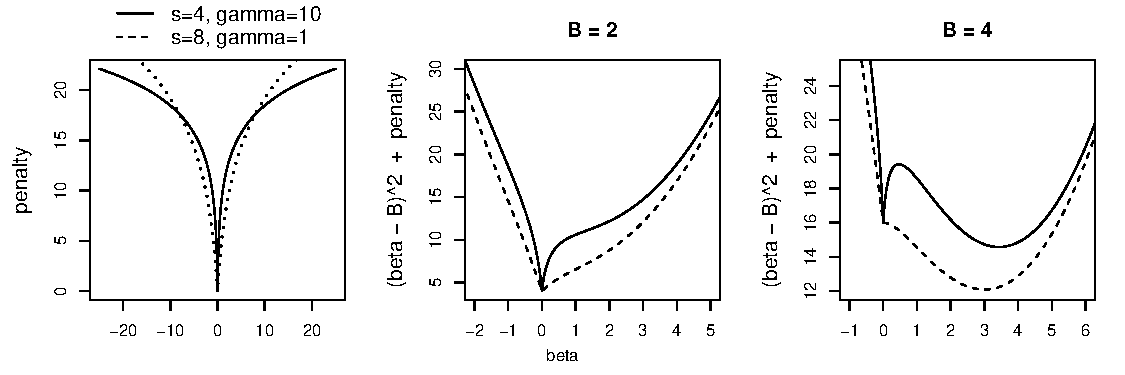
\includegraphics[width=\textwidth]{graphs/solution}
\vskip -.25cm
\caption{\label{solution} Log penalties $c(\beta) = s\log(1 + \gamma|\beta|)$ 
and penalized objectives $(\beta-B)^2 + c(\beta)$.}
\end{figure*}


Concave penalties such as the log penalty, which have a gradient that is
decreasing with absolute coefficient size,  yield the `diminishing-bias'
property discussed above. It is {\it the} reason why one would
use concave penalization instead of $L_1$ or convex alternatives.

Unfortunately, such penalties can overwhelm the convex likelihood and produce a
concave minimization objective; see Figure \ref{solution}.
This  makes computation difficult.  For example,  one run of SCAD via the
\texttt{ncvreg} R package \citep{breheny_coordinate_2011} for the simulation in
Section \ref{sec:sim} requires around 10 minutes, compared to less than a second for 
lasso (or gamma lasso).  The most efficient exact solver that we've found is the
\texttt{sparsenet} of \citet{mazumder_sparsenet_2011}, also implemented in R,
which first fits a lasso path and, for
each segment on this path, adapts coefficient estimates along a second path of
increasing penalty concavity. However, \texttt{sparsenet}  relies upon solution
over a large set of specifications\footnote{POSE shares with
\texttt{sparsenet} the idea of moving along a path of closely related
specifications, but does not require a grid in both  cost size and concavity.
Intuitively,  POSE runs  a path diagonally through this grid.}  
 and its compute cost remains much higher than for the [gamma] lasso.


Local linear approximation \cite[LLA; e.g.,][]{candes_enhancing_2008}
algorithms replace the concave cost function $c$  with its tangent at the
current estimate, $c'(\hat\beta_j)\beta_j$.  The objective is then just a
weighted $L_1$ penalized loss. An exact LLA solver iterates between updating
$c'(\hat\beta)$ and solving the implied $L_1$ penalized minimization problem.
\citet{zou_one-step_2008} present numerical and theoretical evidence that LLA
can provide near-optimal solutions even if you {\it stop it
after one iteration}. This is an example of one-step estimation (OSE), a
technique inspired by \cite{bickel_one-step_1975} that amounts to taking as
your estimator the first step of an iterative approximation to some objective.
Early-stopping can be as good  as the full solution {\it if} the
initial estimates are good enough.

OSE and similar ideas have had a resurgence in the concave penalization
literature recently, motivated by the need for faster estimation algorithms.
\cite{fan_strong_2014} consider early-stopping of LLA for folded concave
penalization  and show that, under strong sparsity assumptions about true
$\bs{\beta}$ and given appropriate initial values, OSE LLA is with high
probability an oracle estimator.   Zhang (2010,2013)
\nocite{zhang_analysis_2010,zhang_multi-stage_2013} investigates  
`convex relaxation' iterations, where estimates under convex regularization
 are the basis for weights in a subsequent penalized objective.
 \cite{wang_calibrating_2013} propose a two step algorithm that feeds lasso
 coefficients into a linear approximation to folded concave penalization.
 These OSE methods are all closely related to  the adaptive lasso
\citep[AL;][]{zou_adaptive_2006}, which does weighted-$L_1$ minimization under
weights $\omega_j = 1/|\hat\beta^0_j|$, where $\hat\beta^0_j$ is an initial
guess at the coefficient value.  The original AL paper advocates using MLE
estimates for initial values, while
\cite{huang_adaptive_2008} suggest using marginal regression coefficients
$\hat\beta^0_j = \mr{cor}(\bm{x}_j,\bm{y})$.

The main point here is that OSE LLA, or a two-step estimator starting from
$\bs{\hat\beta}=0$, or any version of the adaptive lasso, are all  interpretable as weighted-$L_1$ 
penalization with weights equal to something like $c'(\beta^0)$ for initial
coefficient guess $\beta^0$. POSE and GL take advantage of an  available
source of initial values in any path estimation algorithm -- the solved values
from the previous path iteration.  Our  simulations in Section \ref{sec:sim}
show that this efficient strategy works as well or better than  expensive
exact solvers.  In the next section, we provide some theoretical intuition on
why it works.


\subsection{Comparison between weighted-$L_1$ and $L_0$ penalized estimation}


Our oracle benchmark is estimation under $L_0$ costs, $c(\beta_j) =
\ds{1}_{\{\beta_j\neq0\}}$, for which global solution is impractical.   We are
interested in weighted-$L_1$ penalization as a way to obtain fits that are as
sparse as possible without compromising predictive ability, regardless of the
underlying data generating process (or `true' sparsity).

 For  $S \subset \{1\ldots p\}$ with cardinality $|S|=s$ and complement $S^c =
\{1\ldots p\}\setminus S$, denote vectors restricted to covariates in $S$ as
$\bm{\beta}_S = [\beta_j:j\in S]'$, matrices as $\bm{X}_S$, etc.  Use
$\bs{\beta}^S$ to denote the coefficients for ordinary least-squares (OLS)
restricted to $S$: that is, $\bs{\beta}^S_S =
(\bm{X}_S'\bm{X}_S)^{-1}\bm{X}_S'\bm{y}$ and $\beta^{S}_j = 0~\forall~j\notin
S$.  Moreover, $\bm{e}^S = \bm{y}-\bm{X}\bs{\beta}^S =
(\bm{I}-\bm{H}^S)\bm{y}$ are residuals and $\bm{H}^S =
\bm{X}_S(\bm{X}_S'\bm{X}_S)^{-1}\bm{X}_S'$ the projection matrix from OLS on $S$.  
Use $|\cdot|$ and $\|\cdot\|$ for $L_1$ and $L_2$ norms.

We use the following result for iterative \textit{stagewise} regression, with proof in the supplemental appendix. 
\begin{lemma}\label{SSElemma}
Say $\mr{MSE}_S = \|\bm{X}\bs{\beta}^S-\bm{y}\|^2/n$ and 
$\mr{cov}(\bs{x}_j,\bm{e}^S) = \bs{x}_j'(\bm{y}-\bm{X}\bs{\beta}^S)/n$ are sample variance and covariances.  Then for any $j \in 1\ldots p$, 
\[
\mr{cov}^2(\bs{x}_j,\bm{e}^S) \leq \mr{MSE}_S - \mr{MSE}_{S\cup j}
\]
\end{lemma}

In addition, we need to define {\it restricted eigenvalues} (RE) on the gram matrix $\bm{X}'\bm{X}/n$.\footnote{
  This  RE  matches the `adaptive restricted eigenvalues' of \cite{buhlmann_statistics_2011}.  
Similar quantities are common in the theory of regularized estimators; see also
\cite{raskutti_restricted_2010} and  \cite{bickel_simultaneous_2009}.}

  
\begin{definition}\label{redef}
The restricted eigenvalue is
$
\phi^2(L,S) = \min_{\{\bm{v}: \bm{v}\neq \bm{0},~|\bm{v}_{S^c}| \leq L\sqrt{s}\|\bm{v}_S\|\}}\frac{\|\bm{X}\bm{v}\|^2}{n\|\bm{v}\|^2}$.
\end{definition}

Finally,  we bound the distance between prediction rules
from $L_0$ and weighted-$L_1$ penalized estimation.  

\begin{theorem} \label{thm:sparseapprox}  Consider squared-error loss
$l(\bs{\beta}) =
\frac{1}{2}\|\bm{X}\bs{\beta}-\bm{y}\|^2$, and suppose $\bs{\beta}^{\nu}$ minimizes the $L_0$ penalized objective $l(\bs{\beta}) + n\nu\sum_{j=1}^p\ds{1}_{\{\beta_j\neq0\}}$ with $\bs{\beta}^\nu = \bs{\beta}^S$ and $|S|=s<n$.   
Write $\bs{\hat\beta}$ as solution to the weighted-$L_1$ minimization $l(\bs{\beta}) + n\lambda\sum_j\omega_j|\beta_j|$. 

Then  
$\omega^{\mr{min}}_{S^c}\lambda > \sqrt{2\nu}$ while $\phi^2(L,S) > 0$ implies
\begin{equation} \label{sparseineq}
\frac{\|\bm{X}(\bs{\hat\beta}-\bs{\beta}^\nu)\|^2}{n}\leq
\frac{4\lambda^2 \|\bs{\omega}_S\|^2}{\phi^2(L, S)}
\end{equation} 
with 
 $L = \frac{\|\bs{\omega}_S\|}{\sqrt{s}}\left(\omega^{\mr{min}}_{S^c}-\sqrt{2\nu}/\lambda\right)^{-1}$ for the RE.
\end{theorem}

\begin{proof}
From the definitions of $\bs{\hat\beta}$ and $\bs{\beta}^\nu = \bs{\beta}^S$, 
\begin{align}\label{predconv}&
\frac{1}{2}\|\bm{X}\bs{\hat \beta}-\bm{y}\|^2 +  n\lambda\sum_j\omega_j|\hat\beta_j|  \\ &= \frac{\|\bm{X}(\bs{\hat\beta}-\bs{\beta}^\nu)\|^2}{2} + \frac{\|\bm{e}^S\|^2}{2} - \bm{\hat y}'\bm{e}^S+ n\lambda\sum_j\omega_j|\hat\beta_j|\notag\\
&\hspace{3cm}\leq~~\frac{1}{2}\|\bm{e}^S\|^2 + n\lambda\sum_{j\in S}\omega_j|\beta^S_j|\notag
\end{align}
  Since $\bm{\hat y}'\bm{e}^S = \bm{\hat y}'(\bm{I}-\bm{H}^S)\bm{y} =
\bs{\hat\beta}'\bm{X}'(\bm{y}-\bm{X}\bs{\beta}^\nu) = 
\sum_{j\in S^c} \hat\beta_j\bs{x}_j'(\bm{y}-\bm{X}\bs{\beta}^\nu)
$,
 we can apply Lemma \ref{SSElemma} followed by $\bs{\beta}^\nu$ being optimal under $L_0$ penalty $\nu$ to get 
\begin{equation} \label{L0ineq}
\left(\frac{\bs{x}_j'(\bm{y}-\bm{X}\bs{\beta}^\nu)}{n}\right)^2
\leq \mr{MSE}_S - \mr{MSE}_{S\cup j} < 2\nu ~~~\forall~j
\end{equation}
so that $|\bm{\hat y}'\bm{e}^S| = |\bs{\hat\beta}_{S^c}\bm{X}_{S^c}'(\bm{y}-\bm{X}\bs{\beta}^\nu)| < n\sqrt{2\nu}|\bs{\hat\beta}_{S^c}|$.  Applying this inside (\ref{predconv}),
\begin{align}\label{predconvineq}&
\frac{1}{2}\|\bm{X}(\bs{\hat\beta}-\bs{\beta}^\nu)\|^2
  + n\left(\omega^{\mr{min}}_{S^c}\lambda-\sqrt{2\nu}\right)|\bs{\hat\beta}_{S^c}|\\
  &~\leq~ n\lambda\sum_{j\in S}\omega_j|\hat\beta_{j}-\beta^\nu_j|
  ~\leq~ n\lambda\|\bs{\omega}_S\|\|\bs{\hat\beta}_{S}-\bs{\beta}^\nu_S\|.\notag
\end{align}
Given $\omega^{\mr{min}}_{S^c}\lambda > \sqrt{2\nu}$,
difference $\bs{\hat\beta}-\bs{\beta}^\nu$ is in the RE support for 
$L=\frac{\|\bs{\omega}_S\|}{\sqrt{s}}(\omega^{\mr{min}}_{S^c}-\sqrt{2\nu}/\lambda)^{-1}$ and thus $\|\bs{\hat\beta}_{S}-\bs{\beta}^\nu_S\| \leq \|\bm{X}(\bs{\hat\beta}-\bs{\beta}^\nu)/\sqrt{n}\|/\phi(L,S)$.  Finally, applying this inside (\ref{predconvineq}) yields
\begin{align}
\frac{1}{2}\|\bm{X}(\bs{\hat\beta}-\bs{\beta}^\nu)\|^2
  &~\leq~ \frac{\sqrt{n}\lambda\|\bs{\omega}_S\|\|\bm{X}(\bs{\hat\beta}-\bs{\beta}^\nu)\|}
  {\phi(L, S)}.
\end{align}
Dividing each side by $\sqrt{n}\|\bm{X}(\bs{\hat\beta}-\bs{\beta}^\nu)\|/2$ and squaring gives the result.
\end{proof}

\noindent {\bf Remarks}


\noindent $\bullet$~~  Theorem \ref{thm:sparseapprox} is finite sample exact.  Distinguishing it from
related results in the literature, it is  also completely
\textit{non-parametric} -- it makes no reference to the true distribution of
$\bm{y}|\bm{X}$.  Indeed, if we make such assumptions, Theorem
\ref{thm:sparseapprox} provides bounds on the distance between a
weighted-lasso and optimal prediction.  The next remark is an example.

\noindent $\bullet$~~ Assume that $\bm{y} \sim
(\bs{\eta},\sigma^2\bm{I})$ --  $y_i$ independent with mean $\mu_i$ and shared
variance $\sigma^2$.  The $C_p$ formula of
\cite{mallows_comments_1973} gives 
$\mr{MSE}_S + 2s\sigma^2/n$ as an unbiased estimate of residual variance.
Following \cite{efron_estimation_2004}, this implies $\nu = \sigma^2/n$ is the
optimal $L_0$ penalty for minimizing prediction error. Theorem
(\ref{thm:sparseapprox}) applies directly,  with $L =
\frac{\|\bs{\omega}_S\|}{\sqrt{s}}\left(\omega^{\mr{min}}_{S^c}-
\sqrt{2}\sigma/(\lambda\sqrt{n})\right)^{-1}$, to give a bound on the distance
between weighted-$L_1$ estimation and $C_p$-optimal prediction. Note that,
since the condition on minimum $S^c$ weights has become
$\omega^{\mr{min}}_{S^c} > (\sigma/\lambda)\sqrt{2/n}$, comparison to $C_p$
suggests we can use larger $\gamma$  with large $n$ or small $\sigma$.


\noindent $\bullet$~~  Plausibility of the restricted eigenvalue assumption
$\phi(L,S) > 0$ depends  upon $L$.  It is less restrictive if we can reduce
$\|\bs{\omega}_S\|$ without making $\omega^{\mr{min}}_{S_c}$ small.
\textit{This is a key motivation for the POSE algorithm:} if covariates with
nonzero $\hat \beta_j$ for large $\lambda$ (i.e., early in the path) can be
assumed to live in $S$, then increasing $\gamma >0$ will improve prediction.
Of course, the moment that $\lambda$ becomes small enough that elements of
$S_c$ get nonzero $\hat\beta$, then larger $\gamma$ can lead to over-fit.  For
this reason it is essential that we have tools for choosing  optimal
$\lambda$.

\noindent $\bullet$~~ In the supplemental material,  we also adapt standard
results from \cite{wainwright_sharp_2006,wainwright_sharp_2009} to show how
reducing $\|\bs{\omega}_S\|$ without making $\omega^{\mr{min}}_{S_c}$ small
can lead to lower false discovery rates with respect to the $L_0$ oracle.
However, such results depend upon design restrictions that are less realistic
in practice.


\section{Penalty selection}
\label{sec:select}

Lasso, the gamma lasso, and related 
sparse regularization estimators do not actually {\it do} model selection; rather, they
can be used to obtain paths of estimates corresponding to different levels of
penalization.  Each penalty level corresponds to a different `model'
and we must select the optimal choice from these candidates.

$K$-fold cross-validation \cite[CV; e.g.,][]{efron_estimation_2004} 
is the most common technique for penalty selection, and it does a good job.  However, there are many scenarios where
we might want an analytic alternative to CV.  For example, if a single fit is expensive then doing it $K$
times will be impractical.  More subtly, truly Big Data are distributed: they
are too large to store on a single machine. Algorithms can be designed to work
in parallel on subsets
\citep[e.g.,][]{taddy_distributed_2015} but a bottleneck
results if you need to communicate across machines for CV experimentation.
Finally, CV can lead to over-fit for unstable algorithms whose
results change dramatically in response to data jitter; see
\cite{breiman_heuristics_1996} for a classic discussion.  Such instability
arises for large $\gamma$ combined with small $\lambda$ in our GL algorithm
and, more generally, in many concave regularized estimators; see the
supplemental material for a detailed overview.

An important feature of the standard $L_1$ lasso is that it comes with a
simple approximation for the estimation degrees-of-freedom (\textit{df}) at
any $\lambda$: the number of nonzero estimated coefficients
\citep[see][]{zou_degrees_2007}.  These \textit{df} can then combined with the fitted
deviance for penalty selection via common information criteria.

This section derives the gamma lasso as approximately maximizing the posterior
for a hierarchical Bayesian model, and uses this
interpretation to obtain a heuristic degrees-of-freedom for each estimate
along the GL path.  These GL \textit{df} can  be input to information criteria
for model selection. In particular, our extensive simulations demonstrate that the GL
\textit{df} can be used with  the corrected AICc of
\citet{hurvich_regression_1989}  to obtain out-of-sample predictive
performance that is as good or better than that from cross-validated
predictors.


\subsection{Bayesian model interpretation}

Consider a model where each $\beta_j$ is
assigned a Laplace distribution prior with scale $\tau_j>0$,
\begin{equation}\label{blasso}
\beta_j \sim \mr{La}\left(\tau_j\right) =
\frac{\tau_j}{2}\exp\left[ -\tau_j|\beta_j| ~\right].
\end{equation}
Typically, scale parameters $\tau_1 =
\ldots = \tau_p$ are set as a single value, say $n\lambda/\phi$ where
 $\phi$ is the dispersion (e.g. Gaussian variance
$\sigma^2$ or 1 for the binomial).   Posterior
maximization under the prior in (\ref{blasso}) is $L_1$ regularized estimation \citep[e.g.,][]{park_bayesian_2008}.

Instead of a single shared scale, assume an independent gamma
$\mr{Ga}(s,1/\gamma)$ hyperprior with `shape' $s$ and `scale' $\gamma$ for
each $\tau_j$, such that $\ds{E}[\tau_j] = s\gamma$ and $\mr{var}(\tau_j) =
s\gamma^2$.  The {\it joint} coefficient-scale prior is
\begin{align}\label{glprior}
\pi(\beta_j,\tau_j) &= \mr{La}\left(\beta_j ;~ \tau_j\right)
\mr{Ga}\left(\tau_j;~ s,\gamma^{-1}\right) \\&= \frac{ 1}{2\Gamma({s})} 
\left(\frac{\tau_j}{\gamma}\right)^{s}
               \exp\left[-\tau_j(\gamma^{-1}+|\beta_j|)\right].\notag
\end{align}
The gamma hyperprior is conjugate here, implying a $\mr{Ga}\left(s+1, ~1/\gamma +
|\beta_j|\right)$ posterior for $\tau_j \mid \beta_j$ with conditional
posterior mode (MAP) at $\hat\tau_j = \gamma s/(1 + \gamma |\beta_j|)$.

Consider joint MAP estimation of $[\bs{\tau},\bs{\beta}]$ under the prior in
   (\ref{glprior}), where we've suppressed $\alpha$ for simplicity. By taking
   negative logs and removing constants, this is equivalent to solving
\begin{equation}\label{gljoint}
\argmin_{\beta_j\in\ds{R},~\tau_j \in \ds{R}^{+}}\!\!
\frac{l(\bs{\beta})}{\phi} + \sum_j \left[\tau_j(\gamma^{-1}+|\beta_j|) - s\log(\tau_j)\right],
\end{equation}
and is straightforward to show (supplemental) that this is equivalent 
to the log-penalized objective 
\begin{equation}\label{logobj}
\min_{\beta_j\in\ds{R}}~~
\phi^{-1}l(\bs{\beta}) + \sum_j  s\log(1+\gamma|\beta_j|).
\end{equation}

\subsection{Degrees of freedom}


For prediction rules, say $\hat y_i$, that are suitably stable \citep[i.e.,
Lipschitz; see][]{zou_degrees_2007}, the SURE framework of
\cite{stein_estimation_1981} applies and  $df =
\ds{E}\left[\sum_i \partial \hat y_i/\partial y_i\right]$.
Consider  a single coefficient $\beta$ estimated via least-squares under $L_1$
penalty $\tau$.   Write gradient at zero $g = -\sum_i x_iy_i$ and curvature $h
= \sum_i x_i^2$ and set $\varsigma = -{\tt sign}(g)$. The prediction rule is
$\hat y = x(\varsigma/h)(|g|-\tau)_+$ with  derivative $\partial\hat y_i/\partial y = x_i^2/h \ds{1}_{[|g|<\tau]}$, so that the SURE expression
yields $df = \ds{E}\left[ \ds{1}_{[|g|<\tau]} \right]$.   This expectation is
taken with respect to the {\it unknown true} distribution over $\bm{y} |
\bm{X}$, not that estimated from the observed sample.  However, 
 one can evaluate this expression at observed
gradients as an unbiased estimator for the true \textit{df} \citep[e.g.,][]{zou_degrees_2007}.

This motivates our heuristic $df$ in weighted-$L_1$ regularization:  the {\it prior} expectation for the number  $L_1$ penalty dimensions, $\tau_j = \lambda \omega_j$, that are less than their corresponding absolute gradient dimension.  Referring to our Bayesian model above, each $\tau_j$ is $iid$ $\mr{Ga}(s,1/\gamma)$ in the prior,
leading to the GL degrees of freedom
\begin{equation}
\label{edf} df^t = \sum_j \mr{Ga}(|g_{j}|;~n\lambda^t/(\gamma\phi),
1/\gamma), \end{equation} where $\mr{Ga}(~\cdot~;~\mr{shape}, 1/\mr{scale})$
is the Gamma cumulative distribution function and $g_j$ is an estimate of  the
$j^{th}$ coefficient gradient evaluated at $\hat\beta_j=0$.\footnote{Note that the number of unpenalized variables (e.g., 1 for $\alpha$) should also be added to the total  estimation $df$. }

For  orthogonal covariates,  $g_j$ is just the marginal gradient at zero.
In the non-orthogonal case, where $g_{j} = g_j(0)$ becomes a
function of all of the elements of $\bs{\hat\beta}$, we plug in the most recent
$g_j$ at which $\hat\beta^t_j=0$:  this
requires no extra computation and has the advantage of maintaining $df =
\hat p^t$ for $\gamma = 0$.

\subsection{Selection via information criteria}

An information criterion is an attempt to approximate
 divergence between the unknown true data generating
process and our parametric approximation; see the supplement for an
overview.  These  take the form
\begin{equation}
l(\bs{\hat\beta}) + k(df)
\end{equation}
where $k$ is the cost on the degrees-of-freedom associated with
 $\bs{\hat\beta}$ and $l$ is the negative log likelihood.  The AIC of
\cite{akaike_information_1973} uses $k(df) = df$ while the BIC of \cite{schwarz_estimating_1978}
uses $k(df) = \log(n)df/2$.

As detailed in \cite{flynn_efficiency_2013}, the corrected AICc with $k(df) =
df\times n/(n-df-1)$ does a better job than the AIC or BIC in choosing the
optimal model for prediction when $df$ is large.  Alternatively, the BIC is often preferred
for accurate support recovery or avoiding false discovery; see, e.g.,
\cite{zou_degrees_2007}.


\section{Simulation experiment}
\label{sec:sim}

We consider samples of size $n=1000$ from
\begin{align}
\label{simdgp}
&y \sim \mr{N}\left(\bm{x}'\bs{\beta},\sigma^2\right)~\text{where}~\beta_j = \frac{\exp\left(-\frac{j}{\sf d}\right)}{j},~j=1\ldots p,\notag\\
&\text{and}~\bm{x} = \bm{u}*\bm{z},~~\bm{u}\sim \mr{N}\left(\bm{0},\bs{\Sigma}\right),~~z_{j} \stackrel{ind}{\sim} \mr{Bin}(0.5).
\end{align}

\vspace{-.4cm}
\noindent
Each simulation draws means $\eta_i =
\bm{x}_i'\bs{\beta}$, and two response samples (train and test)
$\bm{y},\bm{\tilde y} \sim \mr{N}(\bs{\eta},\sigma^2\bm{I})$. Multicollinearity is
parametrized via $\Sigma_{jk} =
\rho^{|j-k|}$ with $\rho = 0.5$.  We define $\sigma^2$ through {\it signal-to-noise} ratios
$\mr{sd}(\bs{\eta})/\sigma$ of $1/2$, $1$, and $2$; for coefficient decay rates we consider
${\sf d}$ of $10$, $50$, and $100$.

The system in (\ref{simdgp}) is obviously {\it dense}:  true
coefficients are all nonzero.  However, they decay in magnitude along the
index $j$ and
it will be useless to estimate many of them in a $p=n$ regression.
Our sparse oracle comparator is the $C_p$ optimal $L_0$ penalized solution

\vspace{-.75cm}
\begin{equation}\label{l0oracle}
\bs{\beta}^{\star} = \argmin_{\bs{\beta}} \left\{ \|\bm{y}-\bm{X}\bs{\beta}\|^2 + 2\sigma^2\sum_j
\ds{1}_{\{\beta_j\neq0\}}\right\},
\end{equation} which is solvable here by searching through
OLS on $\bm{X}_{\{1\ldots j\}}$ for $j=1\ldots p$ (since coefficients are ordered).

\begin{table}
\vspace{-.2cm}
\footnotesize
\begin{center}
\begin{tabular}{ccc|cc|cc|cc|cc|c|c}
\hline &&&\multicolumn{9}{|c|}{~}\\[-1ex]
\multicolumn{3}{c}{~}&\multicolumn{9}{|c|}{\bf \% Worse than oracle $\boldsymbol{C_p}$  } &   \\[1ex]
& &
& \multicolumn{2}{c}{lasso} 
& \multicolumn{2}{c}{GL $\gamma=1$} 
& \multicolumn{2}{c}{GL $\gamma=10$} 
& \multicolumn{2}{c}{marginal AL} 
& \multicolumn{1}{c|}{~} & \\[-0.5ex]
$\mr{sd}(\bs{\eta})/\sigma$ & {\sf d} & $\rho$ 
& ~~~\scriptsize\it AICc & \multicolumn{1}{c}{\scriptsize\it CV~~~}
& ~~~\scriptsize\it AICc & \multicolumn{1}{c}{\scriptsize\it CV~~~}
& ~~~\scriptsize\it AICc & \multicolumn{1}{c}{\scriptsize\it CV~~~}
& ~~~\scriptsize\it AICc & \multicolumn{1}{c}{\scriptsize\it CV~~~} 
& \multicolumn{1}{c|}{ MCP} & $C_p$ $R^2$ \\[.5ex]
\hline\rule{0pt}{3ex}
& & \it  0  & 3 & 3 & 2 & 2 & 4 & 3 & 2 & 2 & {\bf 1} & \it  0.79 \\
 & \it  10  & \it  0.5  & 5 & 5 & 4 & 3 & 5 & 5 & 8 & 8 & {\bf 2} & \it  0.79 \\
& & \it  0.9  & 7 & 6 & 5 & 5 & 7 & 6 & 10 & 10 & {\bf 3} & \it  0.79 \\[1ex]
\cline{2-3}\rule{0pt}{3ex}
& & \it  0  & 6 & 5 & 5 & {\bf 4} & 6 & 7 & 5 & 5 & {\bf 4} & \it  0.77 \\
\it  2  & \it  50  & \it  0.5  & 11 & 8 & 8 & 7 & 10 & 10 & 14 & 13 & {\bf 5} & \it  0.77 \\
& & \it  0.9  & 14 & 10 & 10 & 8 & 12 & 11 & 45 & 45 & {\bf 7} & \it  0.77 \\[1ex]
\cline{2-3}\rule{0pt}{3ex}
& & \it  0  & 9 & 6 & 7 & 6 & 7 & 8 & 8 & 7 & {\bf 5} & \it  0.75 \\
 & \it  100  & \it  0.5  & 18 & 9 & 11 & {\bf 8} & 12 & 11 & 21 & 17 & 9 & \it  0.75 \\
& & \it  0.9  & 23 & 11 & 13 & {\bf 9} & 14 & 12 & 56 & 56 & 10 & \it  0.75 \\[1ex]
\cline{2-3}\hline\rule{0pt}{3ex}
& & \it  0  & 8 & 8 & 7 & 6 & 14 & 9 & 9 & 10 & {\bf 5} & \it  0.48 \\
 & \it  10  & \it  0.5  & 16 & 16 & 12 & 11 & 20 & 16 & 17 & 17 & {\bf 6} & \it  0.48 \\
& & \it  0.9  & 22 & 22 & 18 & 17 & 27 & 21 & {\bf 9} & {\bf 9} & 10 & \it  0.48 \\[1ex]
\cline{2-3}\rule{0pt}{3ex}
& & \it  0  & 19 & {\bf 17} & {\bf 17} & 18 & 25 & 26 & {\bf 17} & 18 & {\bf 17} & \it  0.44 \\
\it  1  & \it  50  & \it  0.5  & 38 & 32 & 28 & 28 & 30 & 40 & 39 & 38 & {\bf 25} & \it  0.44 \\
& & \it  0.9  & 69 & 68 & 57 & 46 & 70 & 59 & 46 & 46 & {\bf 31} & \it  0.44 \\[1ex]
\cline{2-3}\rule{0pt}{3ex}
& & \it  0  & 26 & {\bf 20} & 24 & 30 & 33 & 51 & 22 & 22 & {\bf 20} & \it  0.40 \\
 & \it  100  & \it  0.5  & 64 & 57 & {\bf 42} & 66 & 45 & 95 & 51 & 47 & 56 & \it  0.40 \\
& & \it  0.9  & 86 & 88 & 89 & 87 & 93 & 89 & {\bf 65} & 66 & 85 & \it  0.40 \\[1ex]
\cline{2-3}\hline\rule{0pt}{3ex}
& & \it  0  & 26 & 27 & 28 & {\bf 23} & 59 & 30 & 43 & 57 & {\bf 23} & \it  0.18 \\
 & \it  10  & \it  0.5  & 49 & 51 & 44 & 41 & 79 & 55 & 69 & 76 & {\bf 28} & \it  0.18 \\
& & \it  0.9  & 44 & 44 & 43 & 42 & 49 & 43 & {\bf 28} & {\bf 28} & 39 & \it  0.18 \\[1ex]
\cline{2-3}\rule{0pt}{3ex}
& & \it  0  & {\bf 53} & 56 & 89 & 82 & 101 & 91 & 72 & 91 & 57 & \it  0.13 \\
\it  0.5  & \it  50  & \it  0.5  & {\bf 90} & 94 & 99 & 98 & 101 & 99 & 106 & 117 & 94 & \it  0.13 \\
& & \it  0.9  & 78 & 79 & 80 & 78 & 88 & 79 & 82 & 80 & {\bf 75} & \it  0.13 \\[1ex]
\cline{2-3}\rule{0pt}{3ex}
& & \it  0  & {\bf 61} & 67 & 106 & 98 & 101 & 100 & 85 & 115 & 68 & \it  0.09 \\
 & \it  100  & \it  0.5  & {\bf 94} & 97 & 101 & 101 & 101 & 101 & 118 & 132 & 98 & \it  0.09 \\
& & \it  0.9  & {\bf 86} & 88 & 91 & 88 & 98 & 90 & 95 & 92 & 87 & \it  0.09 \\[1ex]
\hline
\end{tabular}
\end{center}
\caption{\label{tab:sim} Average out-of-sample $R^2$, reported as  \% worse than the $C_p$ oracle, across 1000 different samples from (\ref{simdgp}).   GL$\gamma$ columns denote {\tt gamlr} with AICc penalty selection, while MCP is {\tt sparsenet} with 5-fold CV selection. The best results are bolded.}
\end{table}


Table \ref{tab:sim} shows  predictive performance, 
measured through out-of-sample (OOS) $R^2 = 1 -
\mr{var}(\bm{\tilde y} - \bm{\hat y})/\mr{var}(\bm{\tilde y})$, for {\tt
gamlr} runs of GL with $\gamma$ of 0 (lasso), 2, and 10. For penalty
selection, we use AICc with the GL $df$ from Section \ref{sec:select}. Results
are compared to the oracle as well as {\tt sparsenet}'s MCP penalized
regression, which applies 5-fold CV to optimize out-of-sample error over a
large grid of potential penalty sizes ($\lambda$) and concavities (analogous
to our $\gamma$).


Note that Table \ref{tab:sim} represents only a small portion of our
simulation study.  The supplemental material includes results for hundreds of
additional configurations: varying levels of sparsity (different $z_i$
distribution) or multicollinearity (different $\bs{\Sigma}$) in $\bm{x}$, as
well as for different prediction algorithms: various CV selection rules, AIC,
and BIC applied to the GL paths as well as to additional adaptive lasso
schemes.  Moreover, the supplement includes results on sensitivity and false
discovery rates with respect to the support used in the oracle $C_p$ scheme,
along with  plots for coefficient estimates, information criteria,
and OOS error rates along $\lambda$.

Insights from the simulations (including supplement):

$\bullet$~~ One of the three GL $\gamma$-specifications is always able to provide performance near to (never more than 1.5\% worse, and sometimes better) that of the computationally intensive routine of CV-selected MCP (over a grid in penalty size and scale).  A single {\tt gamlr} run requires a fraction of a second; {\tt sparsenet} with 5-fold CV requires 15-20 seconds per run.  

$\bullet$~~  AICc and 5-fold CV give roughly the same performance for the GL0 (lasso) and GL2; AICc is often much better than CV for the less stable GL10 paths.  For prediction, AICc is a massive improvement over either BIC or the uncorrected AIC;  the
latter leads to negative $R^2$ in many configurations.

$\bullet$~~  Selected GL2 fits had often half the number of nonzero
coefficients as for the selected lasso fit; GL10 leads to even more sparsity,
sometimes returning less than 10\% of the number of nonzero coefficients given by
lasso.  The results suggest that running {\tt gamlr} with small $\gamma$
(e.g., as in GL2) can provide much additional information compression without
hurting performance.  Even the very sparse $\gamma=10$ fits do nearly as well
as best except in the low signal settings, where all but lasso suffer.
Increasing $\gamma$ also leads to lower false discovery rates with respect to
the $C_p$ oracle.

$\bullet$~~ As $\gamma$ increases, the CV error increases more quickly after
it's minimum; this is predicted by Theorem \ref{thm:sparseapprox}, and indicates that the consequences of over-fit are worse under
faster diminishing-bias. The computation times also increase, although a
single run at $\gamma=10$ still requires less than a second.

$\bullet$~~  Investigation of AICc values finds that minimization of this
criteria {\it across} GL0 and GL2 would have consistently chosen the rule that
does best in Table \ref{tab:sim}.  Thus AICc selection on just two GL paths,
with combined compute time still less than a second,  yields the best or near
best predictor in all scenarios.

\section{Hockey example}
\label{sec:nhl}\vskip -.1cm



\begin{table*}[t]\footnotesize\setstretch{1}
\makebox[\linewidth]{
\begin{tabular}{l|lcc|lcc|lcc|}
\multicolumn{1}{c}{} & \multicolumn{3}{l}{\normalsize \it ~~~$\gamma=0$} & \multicolumn{3}{l}{\normalsize \it ~~~$\gamma=1$} &  \multicolumn{3}{l}{\normalsize \it ~~~$\gamma=10$}\\
%\multicolumn{1}{c}{} & \multicolumn{3}{r|}{} & \multicolumn{3}{r|}{} &  \multicolumn{3}{r|}{}\\
\multicolumn{1}{c}{}  &     &    PPM & PM &    &   PPM & PM        &   & PPM & PM \\
\cline{3-4}\cline{6-7}\cline{9-10}\rule{0pt}{3ex}
1 & Ondrej Palat & 33.8 & 38 & Sidney Crosby & 29.2 & 52 & Sidney Crosby & 32.6 & 52 \\
2 & Sidney Crosby & 31.2 & 52 & Ondrej Palat & 29 & 38 & Jonathan Toews & 22.8 & 35 \\
3 & Henrik Lundqvist & 25.8 & 9 & Jonathan Toews & 21.4 & 35 & Joe Thornton & 22 & 34 \\
4 & Jonathan Toews & 24 & 35 & Joe Thornton & 21 & 34 & Anze Kopitar & 22 & 39 \\
5 & Andrei Markov & 23.1 & 34 & Andrei Markov & 20.9 & 34 & Andrei Markov & 20.7 & 34 \\
6 & Joe Thornton & 21.4 & 34 & Henrik Lundqvist & 19.8 & 9 & Alex Ovechkin & 18.1 & 16 \\
7 & Anze Kopitar & 20.6 & 39 & Anze Kopitar & 19.5 & 39 & Pavel Datsyuk & 16.6 & 13 \\
8 & Tyler Toffoli & 18.9 & 31 & Pavel Datsyuk & 16.1 & 13 & Ryan Getzlaf & 15.8 & 16 \\
9 & Pavel Datsyuk & 17.7 & 13 & Logan Couture & 15.9 & 29 & Henrik Sedin & 15.2 & 7 \\
10 & Ryan Nugent-hopkins & 17.4 & 18 & Alex Ovechkin & 15.8 & 16 & Marian Hossa & 14.9 & 21 \\[-1ex]
\multicolumn{1}{c}{} & \multicolumn{3}{r|}{} & \multicolumn{3}{r|}{} &  \multicolumn{3}{r|}{}\\
 \multicolumn{1}{c}{} & \multicolumn{3}{r|}{\it 305 nonzero effects} & \multicolumn{3}{r|}{\it 204 nonzero effects} &  \multicolumn{3}{r|}{\it 64 nonzero effects}
\end{tabular}}
\caption{\label{nhleffects} Top 10 AICc selected player `partial plus-minus' (PPM) values for the 2013-2014 season.}
\end{table*}

We close with an example analysis: measuring the
performance of hockey players.  It extends  analysis in
\cite{gramacy_estimating_2013,gramacy_hockey_2015}.  The  data include every goal in the National Hockey League (NHL) back to the
2002-2003 season: 69,449 goals and 2439 players.


For goal $i$ in
season $s$ with away team $a$ and home team $h$, say that $q_{i}$ is the probability that the home team scored this goal.  Our regression model is then
\begin{align}\label{hockeymod}
\mr{logit}\left[q_{i}\right] = \alpha_0 +
\alpha_{sh} - \alpha_{sa} + \bm{u}_i'\bs{\phi} + \bm{x}_i'\bs{\beta}_0 +
\bm{x}_i'\bs{\beta}_s, \end{align}  Vector $\bm{u}_i$ holds indicators for
various special-teams scenarios (e.g., a home team power play), and
$\bs{\alpha}$ provides matchup/season specific intercepts. Vector $\bm{x}_i$
contains player effects: $x_{ij}=1$ if player $j$ was on the home team and on
ice for goal $i$, $x_{ij}=-1$ for away player $j$ on ice for goal $i$, and
$x_{ij}=0$ for everyone not on the ice.   Coefficient $\beta_{0j} +
\beta_{sj}$ is the season-$s$ effect of player $j$ on the log odds that, given
a goal has been scored, the goal was scored by their team.  These effects are
`partial' in that they control for who else was on the ice, special teams
scenarios, and team-season fixed effects -- a player's $\beta_{0j}$ or $\beta_{sj}$
only need be nonzero if that player effects play above or below the team
average for a given season.

We estimate GL paths of $\bs{\hat\beta}$ from (\ref{hockeymod}) with
$\bs{\alpha}$ and $\bs{\phi}$ left {\it unpenalized}. Coefficient costs are
{\it not} scaled by covariate standard deviation, since this would have
favored players with little ice time.   The AICc surface
is shown in Figure \ref{nhlic}; it selects denser models with low $\lambda$ but
not-to-big $\gamma$.  See the supplement for additional study, including comparison to BIC and CV.


\begin{figure}[h]
\begin{center}
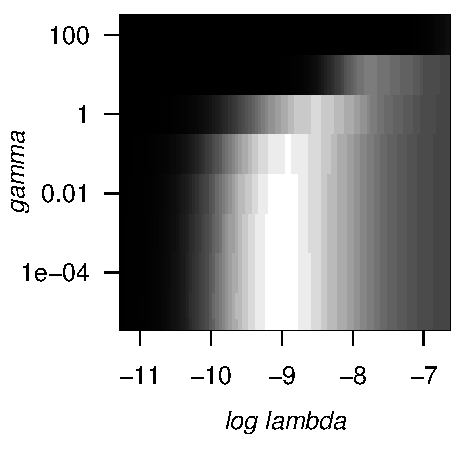
\includegraphics[width=0.35\textwidth]{graphs/nhl_aicc}
\vskip -.4cm
\caption{ \label{nhlic} Hockey AICc, rising from white to black.
}
\end{center}
\vskip -.25cm
\end{figure}

The original goal with this dataset was to build a better version of
hockey's `plus-minus' (PM) statistic: number of goals {\it for} minus {\it
against} each player's team while he is on the ice. To convert from player
effects $\beta_{0j} + \beta_{sj}$ to the scale of `plus/minus', set the probability that a goal was scored by his team given player
$j$ is on ice  (and no other information) as $p_j = e^{\beta_j}/(1+e^{\beta_j})$. The `partial
plus/minus' (PPM) is 
\begin{equation}
 \mr{ppm}_j = N_j(p_j - (1-p_j)) = N_j(2p_j-1)
 \end{equation}  where
$N_j$ is the  number of goals for which he was on-ice.  This measures 
quality and quantity of contribution and lives on the same scale as PM.

Table \ref{nhleffects} contains the estimated PPM values for the 2013-2014
season under various $\gamma$ levels, using AICc selection.  We see that, even
if changing concavity ($\gamma$) has little effect on minimum CV errors (see supplement),
larger $\gamma$  yield more sparse models and different conclusions about
player contribution. At the $\gamma=0$ lasso, there are 305 nonzero player
effects (individuals measurably different from their team's average ability)
and the list includes young players who have had very strong starts to their
careers.  For example, Ondrej Palat and Tyler Toffoli both played their first
full seasons in the NHL in 2013-2014.  As $\gamma$ increases to 1, these young
guys  drop in rank while more proven stars (e.g., Sidney Crosby and Jonathan
Toews) move up the list.  Finally, at $\gamma=10$ only big-name stars remain
amongst the 64 nonzero player effects.


\section{Discussion}
\label{discussion}


Concave penalized estimation for Big Data, where exact solvers are too
 expensive, reduces largely to weighted-$L_1$ penalization.
Path adaptation is an intuitively reasonable source of weights, and we are able to show that POSE -- particularly {\tt gamlr} with AICc selection -- provides diminishing-bias sparse compressed sensing
no more cost than a  standard lasso.  We know of no other software that meets this standard.



\setstretch{1}
\bibliographystyle{chicago}
\bibliography{pose}

\end{document}
